\begin{homeworkProblem}
  Observe que
  \begin{align*}
    I=\int_{0}^{1}\frac{4}{1+x^2}=\pi 
  \end{align*}
  \begin{enumerate}
    \item Use las reglas compuestas del punto medio, del trapecio y de Simpson para aproximar $I$ para varios tamaños de paso de integración $h= \frac{1}{n}, n = 10,50, 100, 250, 500, 1000, 1500, 2000$. Grafique el logaritmo del error absoluto versus $n$ para cada paso. Describa el efecto de redondeo de los errores cuando $i\to 0$.
      \begin{solucion}
        Veamos lo que sucede para cada caso:
        \begin{itemize}
          \item Punto Medio.\\
            Note que al aplicar el algoritmo para la integral obtenemos la siguiente gráfica de errores:
            \begin{figure}[H]
            \begin{center}
              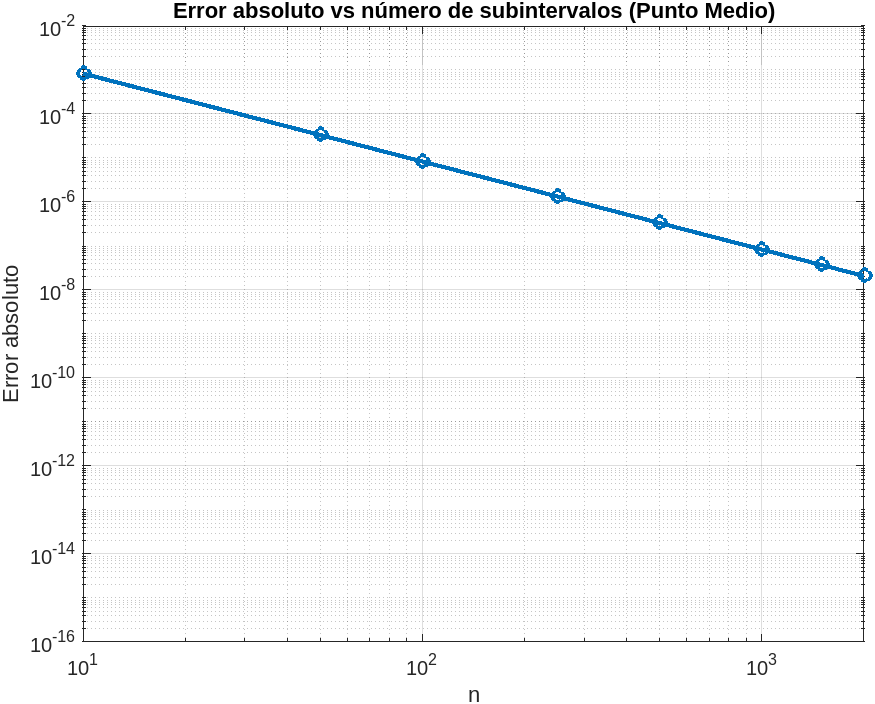
\includegraphics[scale=0.7]{Figures/puntomedio.png}
            \end{center}
            \caption{Error absoluto en el método del punto medio.}
            \end{figure}
            Aquí cabe recordar que el método del punto medio tiene convergencia de orden $O(h^2)$ y su implementación es bastante sencilla, la podremos ver en el siguiente código que aplicando el método se tomo $0.001995$ segundos.
            \newpage
            \lstinputlisting[language=Matlab]{scripts/puntomedio.m}
            \newpage
          \item Trapecio.\\
            Note que al aplicar el algoritmo para la integral obtenemos la siguiente gráfica de errores:
            \begin{figure}[H]
            \begin{center}
              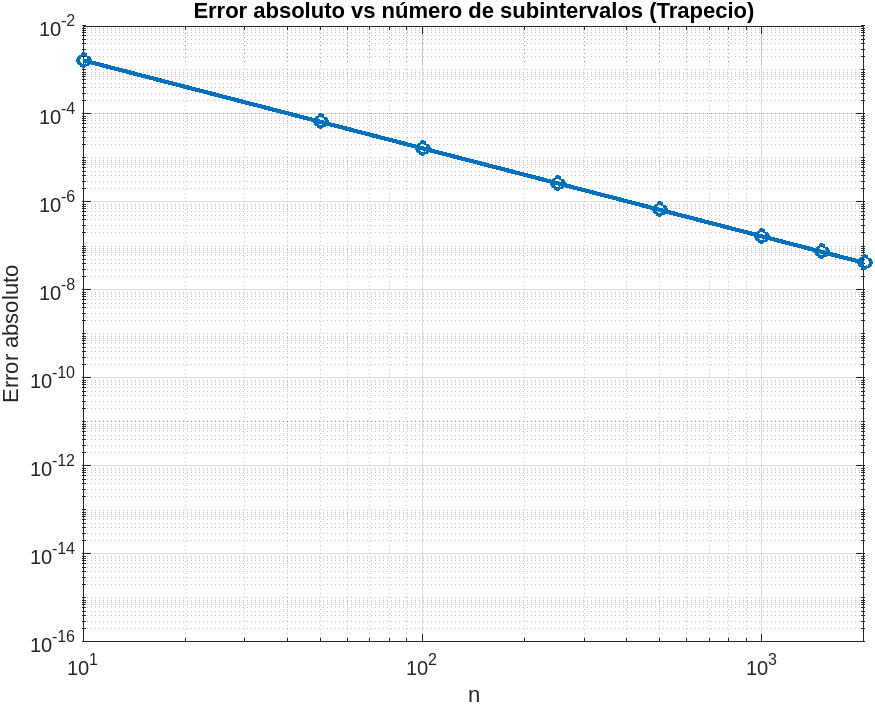
\includegraphics[scale=0.7]{Figures/trapecio.png}
            \end{center}
            \caption{Error absoluto en el método del trapecio.}
            \end{figure}
            Aquí cabe recordar que el método del trapecio tiene convergencia de orden $O(h^2)$ y su implementación es (en cuestiones de operaciones) sencilla, la podremos ver en el siguiente código que aplicando el método se tomo $0.002719$ segundos.
            \newpage
            \lstinputlisting[language=Matlab]{scripts/trapecio.m}
            \newpage
          \item Simpson.\\
            Note que al aplicar el algoritmo para la integral obtenemos la siguiente gráfica de errores:
            \begin{figure}[H]
            \begin{center}
              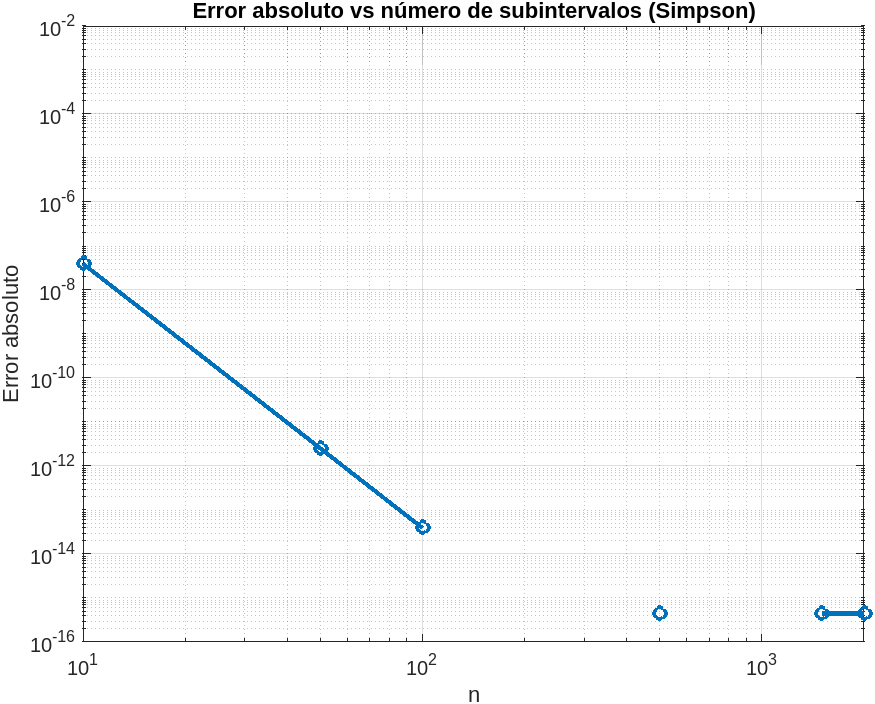
\includegraphics[scale=0.7]{Figures/simpson.png}
            \end{center}
            \caption{Error absoluto en el método de Simpson.}
            \end{figure}
            Aquí cabe recordar que el método tiene convergencia de orden $O(h^4)$ y su implementación es aunque un poco más compleja en la teoría, sigue siendo eficiente cuando hablamos computacionalmente, la podremos ver en el siguiente código que aplicando el método se tomo $0.003878$ segundos.
            \newpage
            \lstinputlisting[language=Matlab]{scripts/simpson.m}
            \newpage
        \end{itemize}
        Ahora sería interesante ver la comparación entre los $3$ métodos en la siguiente figura y la tabla de tiempos:
        \begin{figure}[H]
        \begin{center}
          \includegraphics[scale=0.7]{Figures/comparacion.png}
        \end{center}
        \caption{Comparación de los métodos.}
        \end{figure}
        \begin{center}
        \begin{tabular}{|c|c|}
          \hline
          Método & Tiempo ($s$)\\
          \hline
          Punto medio & $0,001995$\\
          \hline
          Trapecio & $0,002719$\\
          \hline
          Simpson & $0,003878$\\
          \hline
        \end{tabular}
        \end{center}
        De lo que podemos concluir lo siguiente:
        \begin{itemize}
          \item En la aplicación el método del punto medio aparenta ser superior al método del trapecio en cuestiones de errores y tiempo, no obstante la diferencia entre estos aparenta ser bastante baja para tenerlo en cuenta a la hora de realizar los cálculos y favorecer alguna de las $2$, por lo que no se descarta que el uso del método del trapecio sea más efectivo en otro tipos de problemas en los que quizás sea mejor considerar los términos de borde en la función.
          \item Es claro que el método de Simpson es mucho más preciso al momento de aproximar el resultado, pues, desde la propia teoría (la convergencia en orden $O(h^4)$) vimos que al refinar la malla el error se reduciría bastante rápido, por lo que vemos que rápidamente con tomar $n=250$ ya este había superado la precisión numérica de maquina al ser tan cercano a $0$ el error absoluto, situación que con los otros $2$ métodos no se alcanzó a concluir de igual forma.
          \item Si bien en cuestión de tiempo vemos que aún podríamos permitirles a los métodos tener un refinamiento de malla aún más grande, es claro que al método de Simpson le fue suficiente con muy poco y que a los restantes $2$ métodos aparenta aún faltarle mucho al refinamiento de la malla para alcanzar la precisión numérica que tiene el método de Simpson. 
        \end{itemize}
      \end{solucion}
    \item Implemente el método de integración de Romberg para calcular $I$. Grafiqué el logaritmo del error en los términos diagonales en la tabla de extrapolación versus $log(h)$. Verifique sus resultados con la teoría.
      \begin{solucion}
        Note que al aplicar el algoritmo para la integral obtenemos la siguiente gráfica de errores:
        \begin{figure}[H]
        \begin{center}
          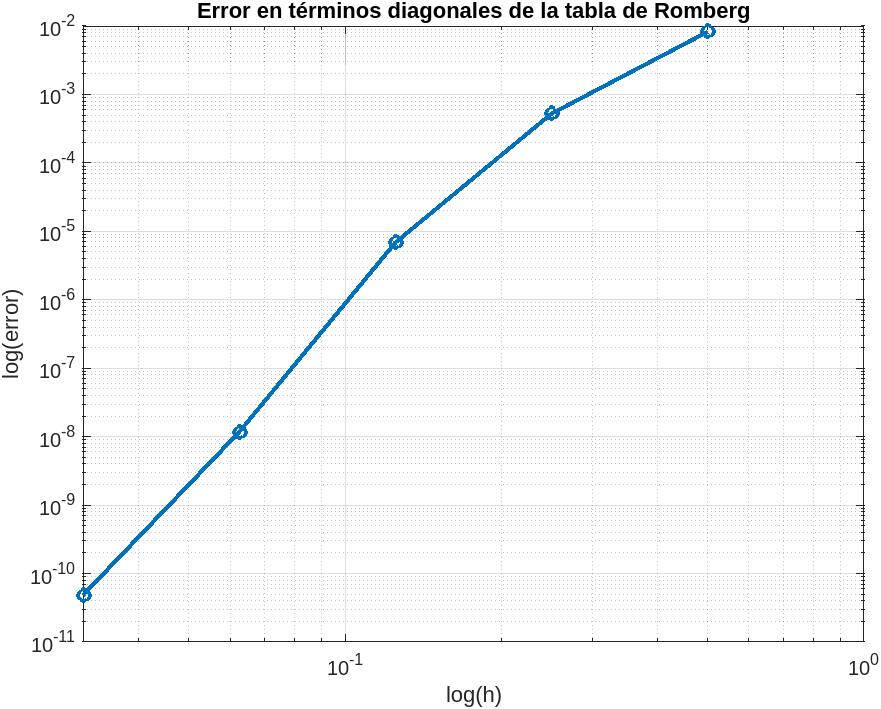
\includegraphics[scale=0.7]{Figures/Romberg.png}
        \end{center}
        \caption{Error en los términos diagonales en la tabla de extrapolación versus $log h$.}
        \end{figure}
        El cuál se tardó $0.004838$ segundos en ejecutarse.
        \newpage
        De aquí podemos concluir lo siguiente:
        \begin{itemize}
          \item Respecto a la teoría, en efecto a valores pequeños de $h$ mejora la aproximación del valor de la integral (más refinamiento, mejor aproximación).
          \item Note que la curva es "casi" una recta, de lo cuál podemos deducir al estar en escala logaritmica que el error $E(h)\approx Ch^{p}$ en donde el valor de $p$ aumenta cada vez más con cada nivel de la extrapolación.
          \item Se alcanzan errores de hasta $10^{-10}$, lo que indica que el método logra una precisión bastante alta con relativamente pocas iteraciones.
        \end{itemize}
        A continuación podemos ver la matriz:
        \begin{align*}
          \begin{pmatrix}
            3.00000000 & 0 & 0 & 0 & 0 & 0\\
            3.10000000 & 3.13333333 & 0 & 0 & 0 & 0\\
            3.13117647 & 3.14156863 & 3.14211765 & 0 & 0 & 0\\
            3.13898849 & 3.14159250 & 3.14159409 & 3.14158578 & 0 & 0\\
            3.14094161 & 3.14159265 & 3.14159266 & 3.14159264 & 3.14159267 & 0\\
          3.14142989 & 3.14159265 & 3.14159265 & 3.14159265 & 3.14159265 & 3.14159265
          \end{pmatrix}
        \end{align*}
        Y en la siguiente página se podrá encontrar el código.
        \newpage
        \lstinputlisting[language=Matlab]{scripts/Romberg.m}
      \end{solucion}
  \end{enumerate}
\end{homeworkProblem}
